\documentclass[11pt,a4paper]{article}

\usepackage[utf8]{inputenc}
\usepackage[T1]{fontenc}
\usepackage{lmodern}
\usepackage[margin=2.4cm]{geometry}
\usepackage{microtype}
\usepackage{amsmath}
\usepackage{booktabs}
\usepackage{enumitem}
\usepackage{csquotes}
\usepackage{fancyvrb}
\usepackage{xcolor}
\usepackage{tcolorbox}
\usepackage{tikz}
\usepackage{pgfplots}
\pgfplotsset{compat=1.18}
\usepgfplotslibrary{groupplots}
\usepackage[authoryear,round]{natbib}
\usepackage[colorlinks=true,linkcolor=blue!50!black,citecolor=blue!50!black,urlcolor=blue!50!black]{hyperref}

\setlist{itemsep=2pt,topsep=4pt}

% One colour per idea, used in every figure.
\definecolor{nearcol}{HTML}{2E8B57}   % near hints (green)
\definecolor{farcol}{HTML}{1F5FAD}    % far hints (blue)
\definecolor{edgecol}{HTML}{E07B00}   % "stopped at the edge" prediction (orange)
\definecolor{basecol}{HTML}{7F7F7F}   % no hint (grey)
\definecolor{selfcol}{HTML}{8E44AD}   % Study 2: self-generated starting point (purple)
\definecolor{givencol}{HTML}{16A085}  % Study 2: given starting point (teal)

\pgfplotsset{
  pilot/.style={
    width=0.62\textwidth, height=5.4cm,
    xtick={0,1,2}, xticklabels={off,low,high}, xmin=-0.3, xmax=2.3,
    xlabel={reasoning level}, legend cell align=left,
    legend style={font=\small, draw=none, fill=white, fill opacity=0.85, text opacity=1},
    tick label style={font=\small}, label style={font=\small},
  },
  witherr/.style={thick, mark=*, mark size=2pt, error bars/y dir=both, error bars/y explicit},
}

\title{\textbf{Pilot Run 1: What We Did and What We Saw}\\[4pt]
\large The first pilot of\\
\emph{Adjusting or Retrieving? Testing the Mechanisms of Anchoring in LLMs}}
\author{Hannan Seyfi\\[8pt]
\normalsize Supervised by Dr.\ Shiva Kamkar (Assistant Professor)\\
\normalsize and Dr.\ Babak Majidi (Associate Professor)\\[8pt]
\normalsize Khatam University}
\date{October 2026}

\begin{document}
\maketitle

\begin{tcolorbox}[colback=yellow!8, colframe=orange!60, title=\textbf{Correction (30 October 2026)}, fonttitle=\normalsize]
With thinking off, this model usually left out the requested \texttt{Estimate:} line. The first version of this report then used the last number in the reply, which was often the anchor repeated back (\enquote{about 121,100 people \ldots\ lower than 192,880,557} was read as 192,880,557) or a year from a refusal (\enquote{as of 2024}). All numbers below now count only replies with the \texttt{Estimate:} line. The thinking-off anchoring index drops from 0.82 to 0.58 (near anchors, 10 questions); the thinking-on values change by less than 0.01.
\end{tcolorbox}

\begin{tcolorbox}[colback=gray!6, colframe=gray!50, title=\textbf{At a glance}, fonttitle=\normalsize]
\begin{itemize}[leftmargin=*]
  \item \textbf{What ran:} a small test model (DeepSeek-R1-Distill-Qwen-1.5B) answered 30 estimation questions at three reasoning levels. That gave 7,200 answers, collected in about 40 minutes on a Colab T4 GPU.
  \item \textbf{The method works from start to finish:} questions go to the model, every answer is saved to GitHub, and the analysis, tables and figures are produced automatically.
  \item \textbf{Anchoring is clear:} anchoring index 0.58 for near anchors with thinking off (about 0.5 in a classic study of people), but that rests on only 10 questions, because without thinking the model rarely gave a proper answer. With thinking it was 0.36 (low) and 0.44 (high). More reasoning (\enquote{high} vs \enquote{low}) does not reduce it further.
  \item \textbf{First mechanism signal:} reading the model's thinking shows that the anchor acts when the model first recalls a value. It either recalls its own value or treats the anchor as something it remembers. Step-by-step adjustment away from the anchor appeared in only 1 of 40 thinking traces.
  \item \textbf{Individual answers are all-or-nothing:} the model mostly either ignores the anchor or copies it.
  \item \textbf{Study 2 is inconclusive:} this model does not know the facts the questions rely on.
  \item \textbf{Main problem found:} the \enquote{high} level barely made the model think longer than \enquote{low} (about 550 vs 430 tokens), because the model stops by itself.
  \item \textbf{Caveat:} a 1.5B model is a test of the method. None of this is a result yet.
\end{itemize}
\end{tcolorbox}

% =====================================================================
\section{What the project asks}
% =====================================================================

When people guess a number right after seeing another number, their guess moves towards it, even when that number is obviously irrelevant. This is the \emph{anchoring effect} \citep{tversky1974judgment}. Large language models (LLMs) show it too. The project asks \emph{why}. Psychology offers two explanations, and they make different predictions:

\begin{description}[leftmargin=1.2em]
  \item[Adjusting] \citep{tversky1974judgment,epley2006anchoring}. You start at the anchor and walk towards your own idea of the answer, but you stop as soon as the number feels acceptable. \emph{Prediction:} answers pile up at the edge of what seems plausible, however far away the anchor was.
  \item[Retrieving] \citep{strack1997explaining,mussweiler1999hypothesis}. The anchor makes you think of facts that fit it (\enquote{11,000 metres? The tallest waterfalls are enormous}), and your whole guess shifts. \emph{Prediction:} answers move by a similar share of the distance, whether the anchor is near or far.
\end{description}

\noindent Reasoning models write out their thinking before they answer, so we can also watch the process, not just the final number. A second question (Study~2) builds on \citet{epley2001putting} and \citet{epley2005effortful}: in people, extra effort (such as being paid for accuracy) helps when you came up with the starting number yourself, but not when someone handed it to you. Does the same hold for LLMs?

% =====================================================================
\section{What we did}
% =====================================================================

\paragraph{The model and the reasoning levels.} The model was DeepSeek-R1-Distill-Qwen-1.5B, a small reasoning model chosen only to test the method on a free GPU. Each question was asked at three \emph{reasoning levels}, which cap how long the model may think before answering: \textbf{off} (no thinking), \textbf{low} (up to 512 tokens) and \textbf{high} (up to 2,048 tokens). A token is roughly three quarters of a word. If the model has not finished thinking when it reaches the cap, we stop it and ask for the answer.

\paragraph{Step 1: find the model's normal zone.} We asked each of 15 questions 60 times with no anchor (20 times per level), for example \enquote{How tall is Angel Falls in Venezuela?} The middle 90\% of its answers (from the 5th to the 95th percentile) is the model's \emph{normal zone} for that question. Anchors are placed relative to this zone, so they are equally surprising for every model.

\paragraph{Step 2: show anchors (Study 1).} We asked the same questions again, but first asked whether the answer is higher or lower than a given number, the classic two-step design \citep{jacowitz1995measures}. Each question got eight anchors:
\begin{itemize}
  \item \textbf{below} or \textbf{above} the normal zone;
  \item \textbf{near} (a quarter of the zone's width beyond its edge) or \textbf{far} (a full zone-width beyond its edge), measured on a log scale;
  \item \textbf{round} (e.g.\ 11,000) or \textbf{precise} (e.g.\ 11,180), because precise anchors are known to pull people harder \citep{janiszewski2008precision}.
\end{itemize}
Each anchor was asked 10 times per level. This is the exact message the model saw for one of them:

\begin{Verbatim}[frame=single, fontsize=\small, framesep=3mm]
How tall is Angel Falls in Venezuela?

First, is it higher or lower than 11,000 metres? Then give your best
estimate. End your reply with these two lines:
Comparison: <higher or lower>
Estimate: <number>
where <number> is a single number in metres (not a range).
\end{Verbatim}

\paragraph{Study 2: who supplies the starting number?} Fifteen different questions each have a familiar but wrong starting value, for example \enquote{What is the normal body temperature of a healthy adult chicken?} The familiar value is 37\,\textdegree C (a human's temperature); the true value is 41.5\,\textdegree C. In the \textbf{self} condition we simply ask, so the model must think of 37\,\textdegree C by itself. In the \textbf{given} condition we first ask \enquote{higher or lower than 37\,\textdegree C?}. Each version was asked with no extra instruction, with \enquote{accuracy matters}, and with \enquote{consider reasons why the true value might be different} \citep{mussweiler2000overcoming}.

\begin{table}[ht]
\centering\small
\begin{tabular}{lrp{8cm}}
\toprule
Part & Answers & What varies \\
\midrule
Normal zone (baseline) & 900 & 15 questions $\times$ 3 levels $\times$ 20 \\
Study 1 (anchors) & 3,600 & 15 questions $\times$ 8 anchors $\times$ 3 levels $\times$ 10 \\
Study 2 (self vs given) & 2,700 & 15 questions $\times$ 2 sources $\times$ 3 instructions $\times$ 3 levels $\times$ 10 \\
\midrule
Total & 7,200 & \\
\bottomrule
\end{tabular}
\caption{Size of the pilot for one model.}
\end{table}

% =====================================================================
\section{One question up close: Angel Falls}
% =====================================================================

Figure~\ref{fig:angel} shows every answer to one question at the \enquote{low} reasoning level. The true height is 979\,m, and the model knows it roughly: with no anchor, most answers were close to 980\,m, and its normal zone runs from 310 to 5,555\,m.

\begin{figure}[ht]
\centering
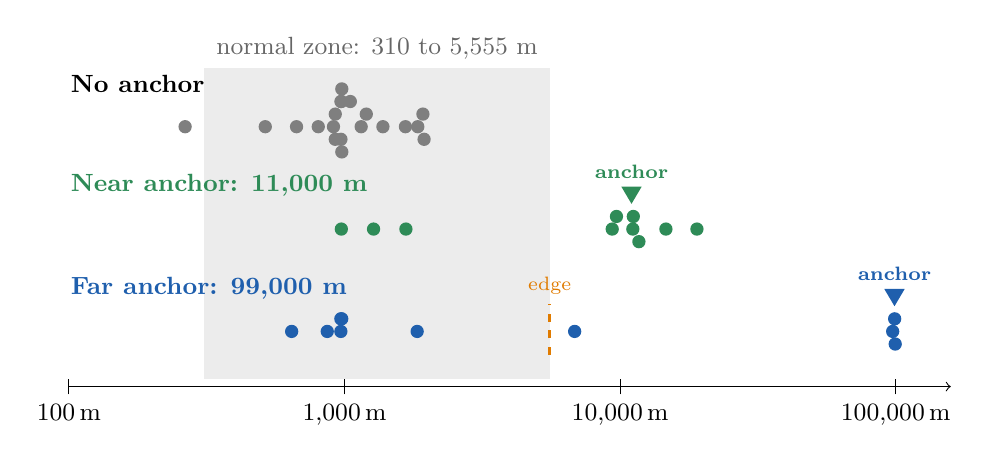
\begin{tikzpicture}[x=1cm,y=1cm]
  % normal zone
  \fill[basecol!15] (1.722,0.0) rectangle (6.106,3.95);
  \node[font=\small, text=basecol!80!black] at (3.914,4.2) {normal zone: 310 to 5,555 m};
  % orange: where far answers would stop under "adjusting"
  \draw[edgecol, very thick, dashed] (6.106,0.3) -- (6.106,0.95);
  \node[font=\scriptsize, text=edgecol, above] at (6.106,0.95) {edge};
  % row labels
  \node[anchor=west, font=\small\bfseries] at (-0.1,3.75) {No anchor};
  \node[anchor=west, font=\small\bfseries, text=nearcol] at (-0.1,2.45) {Near anchor: 11,000 m};
  \node[anchor=west, font=\small\bfseries, text=farcol] at (-0.1,1.15) {Far anchor: 99,000 m};
  % anchors: a triangle above each row points at the anchor value
  \fill[nearcol] (7.145,2.22) -- ++(-0.13,0.22) -- ++(0.26,0) -- cycle;
  \node[font=\scriptsize\bfseries, text=nearcol, above] at (7.145,2.42) {anchor};
  \fill[farcol] (10.485,0.92) -- ++(-0.13,0.22) -- ++(0.26,0) -- cycle;
  \node[font=\scriptsize\bfseries, text=farcol, above] at (10.485,1.12) {anchor};
  % answers
  \fill[basecol] (1.476,3.20) circle (2.4pt);
  \fill[basecol] (2.494,3.20) circle (2.4pt);
  \fill[basecol] (2.891,3.20) circle (2.4pt);
  \fill[basecol] (3.167,3.20) circle (2.4pt);
  \fill[basecol] (3.360,3.20) circle (2.4pt);
  \fill[basecol] (3.383,3.36) circle (2.4pt);
  \fill[basecol] (3.383,3.04) circle (2.4pt);
  \fill[basecol] (3.455,3.04) circle (2.4pt);
  \fill[basecol] (3.455,3.52) circle (2.4pt);
  \fill[basecol] (3.460,3.52) circle (2.4pt);
  \fill[basecol] (3.466,2.88) circle (2.4pt);
  \fill[basecol] (3.466,3.68) circle (2.4pt);
  \fill[basecol] (3.574,3.52) circle (2.4pt);
  \fill[basecol] (3.712,3.20) circle (2.4pt);
  \fill[basecol] (3.777,3.36) circle (2.4pt);
  \fill[basecol] (3.988,3.20) circle (2.4pt);
  \fill[basecol] (4.274,3.20) circle (2.4pt);
  \fill[basecol] (4.431,3.20) circle (2.4pt);
  \fill[basecol] (4.496,3.36) circle (2.4pt);
  \fill[basecol] (4.511,3.04) circle (2.4pt);
  \fill[nearcol] (3.460,1.90) circle (2.4pt);
  \fill[nearcol] (3.869,1.90) circle (2.4pt);
  \fill[nearcol] (4.280,1.90) circle (2.4pt);
  \fill[nearcol] (6.900,1.90) circle (2.4pt);
  \fill[nearcol] (6.954,2.06) circle (2.4pt);
  \fill[nearcol] (7.162,1.90) circle (2.4pt);
  \fill[nearcol] (7.168,2.06) circle (2.4pt);
  \fill[nearcol] (7.239,1.74) circle (2.4pt);
  \fill[nearcol] (7.582,1.90) circle (2.4pt);
  \fill[nearcol] (7.976,1.90) circle (2.4pt);
  \fill[farcol] (2.829,0.60) circle (2.4pt);
  \fill[farcol] (3.281,0.60) circle (2.4pt);
  \fill[farcol] (3.454,0.60) circle (2.4pt);
  \fill[farcol] (3.454,0.76) circle (2.4pt);
  \fill[farcol] (3.465,0.76) circle (2.4pt);
  \fill[farcol] (4.423,0.60) circle (2.4pt);
  \fill[farcol] (6.423,0.60) circle (2.4pt);
  \fill[farcol] (10.462,0.60) circle (2.4pt);
  \fill[farcol] (10.487,0.76) circle (2.4pt);
  \fill[farcol] (10.494,0.44) circle (2.4pt);
  % axis (log scale: 3.5 cm per factor of ten)
  \draw[->] (0,-0.1) -- (11.2,-0.1);
  \foreach \x/\lab in {0/100, 3.5/{1,000}, 7/{10,000}, 10.5/{100,000}} {
    \draw (\x,-0.2) -- (\x,0.0);
    \node[below, font=\small] at (\x,-0.2) {\lab\,m};
  }
\end{tikzpicture}
\caption{Every answer to \enquote{How tall is Angel Falls?} at the low reasoning level (one dot per answer; true height 979\,m). Grey: no anchor (20 answers). Green: after the near anchor of 11,000\,m (10 answers). Blue: after the far anchor of 99,000\,m (10 answers). Triangles mark the anchors. The orange dashed line marks the edge of the normal zone, where \enquote{adjusting} says far-anchored answers should stop. The axis is logarithmic.}
\label{fig:angel}
\end{figure}

\noindent What the model did:
\begin{itemize}
  \item \textbf{Near anchor (11,000\,m):} 7 of 10 answers jumped to the anchor's neighbourhood (9,366 to 19,000\,m); 3 stayed near its usual answer. One trace reads: \emph{\enquote{I think it's somewhere around 9,366 meters, but I'm not entirely sure.}}
  \item \textbf{Far anchor (99,000\,m):} 6 of 10 answers stayed near the usual answer, 1 landed in between, and 3 simply copied the anchor (97,500 to 99,600\,m). An ignoring trace: \emph{\enquote{I remember hearing that Angel Falls is around 970 meters [\dots] That means it's lower than 99,000 meters.}} A copying trace: \emph{\enquote{I believe it's somewhere around 97,000 to 99,000 meters.}}
\end{itemize}
So for a single answer the anchor tends to win completely or lose completely. The summaries below use the middle (median) answer of each set of 10, which averages over this mix.

% =====================================================================
\section{Results}
% =====================================================================

All numbers below are averaged over the 15 questions. Error bars are 95\% bootstrap intervals over questions, so wide bars mean the questions disagreed.

\subsection{Did the model think more when allowed to?}

\begin{figure}[ht]
\centering
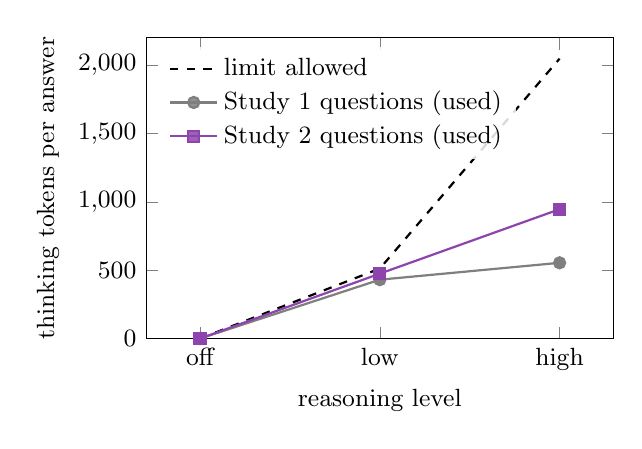
\begin{tikzpicture}
\begin{axis}[pilot, ylabel={thinking tokens per answer}, ymin=0, ymax=2200, legend pos=north west]
  \addplot[black, thick, dashed, mark=none] coordinates {(0,0) (1,512) (2,2048)};
  \addlegendentry{limit allowed}
  \addplot[basecol, thick, mark=*] coordinates {(0,0) (1,430.7) (2,554.2)};
  \addlegendentry{Study 1 questions (used)}
  \addplot[selfcol, thick, mark=square*] coordinates {(0,0) (1,474.9) (2,946.2)};
  \addlegendentry{Study 2 questions (used)}
\end{axis}
\end{tikzpicture}
\caption{How long the model actually thought, against the limit it was given.}
\label{fig:tokens}
\end{figure}

At \enquote{low} the model used most of its 512 tokens and was cut off in about 43\% of Study~1 answers. At \enquote{high} it was allowed 2,048 tokens but used only about 550 on Study~1 questions, because it decided it was done. It thought longer on the Study~2 physics questions (about 950). \textbf{Consequence:} for this model, \enquote{high} is barely different from \enquote{low}, so the pilot cannot yet say whether more thinking helps.

\subsection{Does anchoring appear?}

The \emph{anchoring index} \citep{jacowitz1995measures} compares the answers after a high and a low anchor. For Angel Falls, the near anchors were 11,000 and 150\,m and the median answers 10,414 and 322\,m, so the answers covered 93\% of the gap between the anchors: an index of 0.93. An index of 0 means the anchor changed nothing; 1 means the answers moved as far as the anchors.

\begin{figure}[ht]
\centering
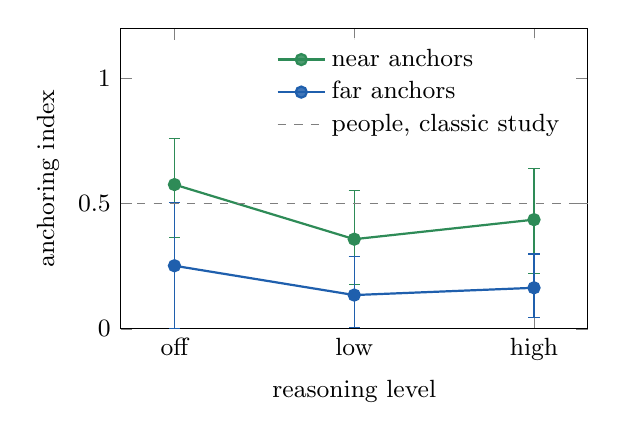
\begin{tikzpicture}
\begin{axis}[pilot, ylabel={anchoring index}, ymin=0, ymax=1.2, legend pos=north east]
  \addplot[nearcol, witherr] coordinates {(0,0.576) += (0,0.185) -= (0,0.210) (1,0.358) += (0,0.193) -= (0,0.180) (2,0.436) += (0,0.205) -= (0,0.214)};
  \addlegendentry{near anchors}
  \addplot[farcol, witherr] coordinates {(0,0.252) += (0,0.251) -= (0,0.249) (1,0.135) += (0,0.153) -= (0,0.128) (2,0.164) += (0,0.135) -= (0,0.118)};
  \addlegendentry{far anchors}
  \addplot[basecol, dashed, mark=none, domain=-0.3:2.3, samples=2] {0.5};
  \addlegendentry{people, classic study}
\end{axis}
\end{tikzpicture}
\caption{Anchoring index by reasoning level.}
\label{fig:index}
\end{figure}

With thinking off, near anchors give an index of 0.58, a little above the 0.49 that \citet{jacowitz1995measures} found for people. Their anchors were chosen differently, so this comparison is rough, and the thinking-off value rests on only 10 questions (most replies without thinking had no \texttt{Estimate:} line). With thinking it is about 0.36 (low) and 0.44 (high). So reasoning may reduce anchoring somewhat but does not remove it, and the higher budget did not help further. This matches what others report \citep{kraishan2026long}, although here \enquote{high} hardly differed from \enquote{low} (Figure~\ref{fig:tokens}). Far anchors give lower values partly by construction: they are further apart, so the same movement is a smaller share of the gap.

\subsection{Adjusting or retrieving?}

This is the main mechanism test. For each anchor we measure the \emph{shift}: how far the median answer moved from the model's usual answer towards the anchor, on a log scale. 0 means no movement; 1 means the answer equals the anchor. For Angel Falls (low level) the near anchor gave a shift of 0.98 and the far anchor 0.08.

The orange line in Figure~\ref{fig:nearfar} is a prediction, not a measurement: the shift the far anchor \emph{would} produce if answers stopped exactly at the edge of the normal zone (for Angel Falls, 5,555\,m, a shift of 0.38).
\begin{itemize}
  \item If the model \textbf{adjusts}, far-anchor answers stop at the edge: the blue line should lie on the orange line.
  \item If the model \textbf{retrieves}, the far anchor shifts answers by the same share as the near one: the blue line should lie on the green line.
\end{itemize}

\begin{figure}[ht]
\centering
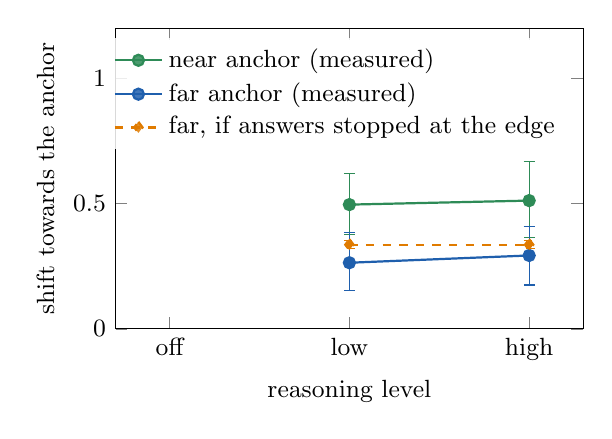
\begin{tikzpicture}
\begin{axis}[pilot, ylabel={shift towards the anchor}, ymin=0, ymax=1.2, legend pos=north east]
  \addplot[nearcol, witherr] coordinates {(1,0.496) += (0,0.125) -= (0,0.118) (2,0.512) += (0,0.155) -= (0,0.147)};
  \addlegendentry{near anchor (measured)}
  \addplot[farcol, witherr] coordinates {(1,0.264) += (0,0.120) -= (0,0.111) (2,0.293) += (0,0.115) -= (0,0.118)};
  \addlegendentry{far anchor (measured)}
  \addplot[edgecol, witherr, dashed, mark=diamond*] coordinates {(1,0.336) += (0,0.017) -= (0,0.015) (2,0.336) += (0,0.015) -= (0,0.014)};
  \addlegendentry{far, if answers stopped at the edge}
\end{axis}
\end{tikzpicture}
\caption{Shift or stop at the edge? For medians, blue on orange would suggest adjusting and blue on green retrieving. The text explains why the medians alone cannot settle it.}
\label{fig:nearfar}
\end{figure}

\noindent\textbf{What we see.} With thinking on, the blue line (0.26 to 0.29) sits at or slightly below the orange line (0.34) and well below the green line (0.50). With thinking off, too few replies had a proper answer to measure this (the \enquote{off} points are left out). On medians alone this looks like adjusting, but reading the model's thinking shows that it is not.

\paragraph{What the thinking shows.} We read 40 randomly chosen thinking traces (anchors above the normal zone, thinking on). In 31 of 40, the first value the model settled on was its final answer. In 23 of these it was the model's own value and the anchor was ignored; in 8 the value it \enquote{remembered} was the anchor itself (Angel Falls, anchor 99,000\,m: \emph{\enquote{I've heard it's around 97,000 meters tall}}). In 4 traces the model recalled its own value and was then pushed towards the anchor. Only 1 trace started at the anchor and corrected part of the way back, the textbook adjusting pattern. So the anchor acts at the moment the model recalls a value, not through gradual adjustment. The low blue line has a simpler cause: far anchors are copied less often than near ones (Table~\ref{tab:copies}), so the median sits lower. This was a first reading by one reader; the planned two-coder reading must confirm it.

\begin{table}[ht]
\centering
\small
\begin{tabular}{llrr}
\toprule
Thinking & Anchor & Stayed in own zone & Copied the anchor \\
\midrule
off  & near & 7\% & 8\% \\
     & far  & 10\% & 4\% \\
low  & near & 54\% & 28\% \\
     & far  & 54\% & 18\% \\
high & near & 51\% & 31\% \\
     & far  & 55\% & 15\% \\
\bottomrule
\end{tabular}
\caption{What single answers did after an anchor above the normal zone (200 answers per row). \enquote{Copied} means within 10\% of the anchor; the rest landed elsewhere or gave no proper answer. With thinking off, 81--82\% of replies had no \texttt{Estimate:} line, so those rows say little.}
\label{tab:copies}
\end{table}

\paragraph{Precise vs round anchors.} Precise anchors (e.g.\ 11,180) shifted answers more than round ones (e.g.\ 11,000), by about 0.10 to 0.12 on the shift scale. The interval excludes zero at the low and high levels (low: $+0.11$, interval $0.01$ to $0.21$; high: $+0.12$, $0.04$ to $0.20$). With thinking off there were too few proper answers to measure it. In people this is explained by adjustment in smaller steps from a precise number \citep{janiszewski2008precision}. In this model part of it may have a simpler cause: some answers borrow the anchor's digits (after a precise anchor of 173,200,000\,km$^2$ for the area of Malta, one answer was 173,000\,km$^2$).

\subsection{Study 2: does thinking help more when the model picks the starting number?}

Here we measure \emph{adjustment}: 0 means the answer stayed at the familiar starting value (such as 37\,\textdegree C), and 1 means it reached the truth. The human prediction \citep{epley2005effortful} is that more thinking raises the purple line (self) but not the teal line (given).

\begin{figure}[ht]
\centering
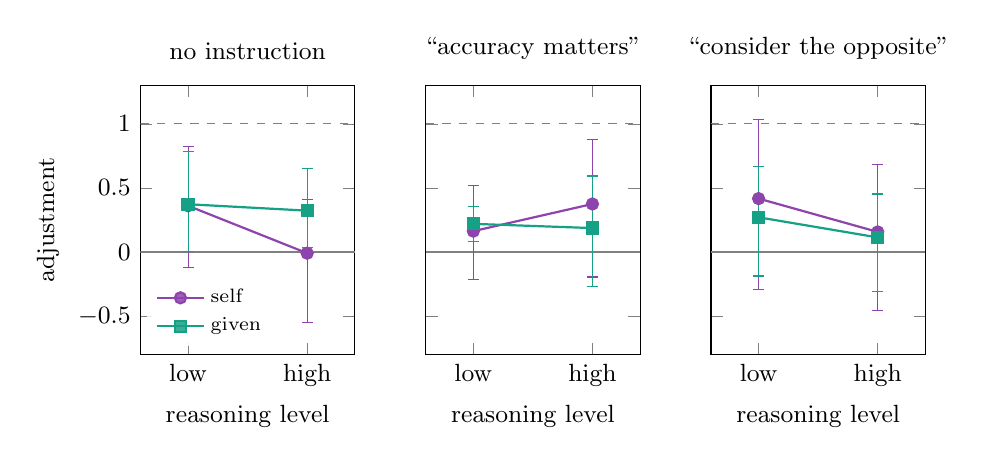
\begin{tikzpicture}
\begin{groupplot}[
  group style={group size=3 by 1, horizontal sep=0.9cm, ylabels at=edge left, yticklabels at=edge left},
  width=0.355\textwidth, height=5cm, xtick={0,1}, xticklabels={low,high}, xmin=-0.4, xmax=1.4,
  ymin=-0.8, ymax=1.3, ylabel={adjustment}, xlabel={reasoning level},
  tick label style={font=\small}, label style={font=\small}, title style={font=\small},
  legend style={font=\scriptsize, draw=none, fill=white, fill opacity=0.85, text opacity=1}, legend cell align=left,
]
\nextgroupplot[title={no instruction}, legend pos=south west]
  \draw[gray, dashed] (axis cs:-0.4,1) -- (axis cs:1.4,1);
  \draw[gray] (axis cs:-0.4,0) -- (axis cs:1.4,0);
  \addplot[selfcol, witherr] coordinates {(0,0.361) += (0,0.464) -= (0,0.483) (1,-0.009) += (0,0.418) -= (0,0.544)};
  \addlegendentry{self}
  \addplot[givencol, witherr, mark=square*] coordinates {(0,0.373) += (0,0.409) -= (0,0.368) (1,0.323) += (0,0.326) -= (0,0.289)};
  \addlegendentry{given}
\nextgroupplot[title={\enquote{accuracy matters}}]
  \draw[gray, dashed] (axis cs:-0.4,1) -- (axis cs:1.4,1);
  \draw[gray] (axis cs:-0.4,0) -- (axis cs:1.4,0);
  \addplot[selfcol, witherr] coordinates {(0,0.163) += (0,0.358) -= (0,0.380) (1,0.375) += (0,0.503) -= (0,0.570)};
  \addplot[givencol, witherr, mark=square*] coordinates {(0,0.220) += (0,0.134) -= (0,0.136) (1,0.187) += (0,0.406) -= (0,0.456)};
\nextgroupplot[title={\enquote{consider the opposite}}]
  \draw[gray, dashed] (axis cs:-0.4,1) -- (axis cs:1.4,1);
  \draw[gray] (axis cs:-0.4,0) -- (axis cs:1.4,0);
  \addplot[selfcol, witherr] coordinates {(0,0.417) += (0,0.614) -= (0,0.709) (1,0.157) += (0,0.524) -= (0,0.613)};
  \addplot[givencol, witherr, mark=square*] coordinates {(0,0.271) += (0,0.396) -= (0,0.458) (1,0.114) += (0,0.339) -= (0,0.419)};
\end{groupplot}
\end{tikzpicture}
\caption{Study 2 adjustment away from the familiar starting value (0) towards the truth (1, dashed). The \enquote{off} level is left out; see the text.}
\label{fig:study2}
\end{figure}

\noindent\textbf{What we see.} Both lines stay between about 0 and 0.4, with wide error bars, and there is no consistent gap between self and given. Example: for the chicken question the model answered about 36 to 37\,\textdegree C at both reasoning levels, whether or not we gave it 37\,\textdegree C. The likeliest reason is that a 1.5B model does not know these facts, so it has nothing to adjust towards. The \enquote{off} level is not shown because its answers were unusable: only 9\% used the \texttt{Estimate:} line (the rest were often refusals) and some were wild, such as $-10$\,\textdegree C for boiling water on a mountain.

\subsection{Data quality}

\begin{table}[ht]
\centering\small
\begin{tabular}{llrrrr}
\toprule
Part & Level & Answers & Gave a number (old reading) & Used the format & Thinking tokens \\
\midrule
Baseline & off & 300 & 91\% & 0\% & 0 \\
 & low & 300 & 100\% & 93\% & 436 \\
 & high & 300 & 100\% & 94\% & 556 \\
Study 1 & off & 1,200 & 90\% & 17\% & 0 \\
 & low & 1,200 & 100\% & 99\% & 431 \\
 & high & 1,200 & 100\% & 98\% & 554 \\
Study 2 & off & 900 & 69\% & 9\% & 0 \\
 & low & 900 & 100\% & 98\% & 475 \\
 & high & 900 & 100\% & 96\% & 946 \\
\bottomrule
\end{tabular}
\caption{\enquote{Gave a number}: a usable estimate could be read from the reply. \enquote{Used the format}: the reply ended with the requested \texttt{Estimate:} line; only these replies are used now. \enquote{Gave a number (old reading)} is what the first version counted: any number in the reply, which with thinking off was often the anchor repeated back or a year from a refusal.}
\end{table}

\begin{itemize}
  \item \textbf{With thinking switched off, this model ignores the answer format and often refuses.} This was expected: R1-distilled models are trained to always think first.
  \item \textbf{Some anchors could not be used.} This model's normal zones were very wide (for London Underground stations, 22 to 57,000), so a few \enquote{far below} anchors came out as 0 or $-1$. These 11 of 120 anchors were left out of the analysis, and the code now refuses to place such anchors.
  \item \textbf{No question was flagged as memorised} (a model that knows the exact answer would show almost no spread). This is expected for a small model and must be checked again with the larger ones.
\end{itemize}

% =====================================================================
\section{What we learned and what comes next}
% =====================================================================

\paragraph{What the pilot shows.} The full pipeline works: prompts, running on Colab, saving to GitHub, and an automatic report. The measures behave sensibly on real model output. Even this small model shows clear anchoring, which reasoning does not remove. Reading its thinking shows that the anchor acts when the model first recalls a value (it recalls its own value or treats the anchor as a memory); step-by-step adjustment was rare (1 of 40 traces).

\paragraph{Next steps.}
\begin{enumerate}
  \item Run the two planned pilot models, Qwen3-8B and DeepSeek-R1-Distill-Llama-8B, on an A100 or L4 GPU.
  \item Make the \enquote{high} level really mean more thinking. One option is to stop the model from ending its thinking early by appending \enquote{Wait} when it tries to stop before the budget, the budget-forcing method of \citet{muennighoff2025s1}.
  \item Analyse individual answers as well as medians, given the all-or-nothing pattern in Figure~\ref{fig:angel}.
  \item Check the true answers of all 30 questions against primary sources.
  \item Hand-code 200 reasoning traces (adjusting / retrieving / dismissing / taking the anchor as a memory) with two coders, to test the trace-based measure.
\end{enumerate}

\paragraph{Points to discuss.}
\begin{itemize}
  \item Is \enquote{copying the anchor} a separate behaviour worth modelling, apart from adjusting and retrieving?
  \item Should far anchors be capped for models whose normal zone is extremely wide?
  \item Is forcing longer thinking (step 2) acceptable as the \enquote{high} condition, or should we rely on each model's own effort settings?
\end{itemize}

\bigskip
\noindent\small Code, data and the automatic report are in the project repository (\texttt{HannanSeyfi/Anchoring-LLMs}): \texttt{results/pilot/summary.md}.

\bibliographystyle{plainnat}
\bibliography{references}

\end{document}
